\documentclass[letterpaper, notitlepage]{revtex4-1}
\usepackage{longtable}
\usepackage{graphicx} 
\usepackage{sidecap}
\usepackage{balance}
\usepackage{amsmath}
\usepackage{amssymb}
\usepackage{amssymb}
\newcommand*{\QEDA}{\hfill\ensuremath{\blacksquare}}%
\newcommand*{\QEDB}{\hfill\ensuremath{\square}}%
\usepackage{siunitx}
\usepackage[none]{hyphenat}
\usepackage[margin=0.7in]{geometry}
\usepackage{esvect}
\usepackage{braket}
\usepackage{listings}
\usepackage{epstopdf}
\usepackage{subfigure}
\usepackage{color} %red, green, blue, yellow, cyan, magenta, black, white
\usepackage{verbatim}
\usepackage{mwe}
\definecolor{mygreen}{RGB}{28,172,0} % color values Red, Green, Blue
\definecolor{mylilas}{RGB}{170,55,241}
\graphicspath{{Figures/}}
\DeclareSIUnit\uvrms{\micro\volt{}_{RMS}}
\DeclareSIUnit\mvrms{\milli\volt{}_{RMS}}

\begin{document}
\lstset{language=Matlab,%
    %basicstyle=\color{red},
    breaklines=true,%
    morekeywords={matlab2tikz},
    keywordstyle=\color{blue},%
    morekeywords=[2]{1}, keywordstyle=[2]{\color{black}},
    identifierstyle=\color{black},%
    stringstyle=\color{mylilas},
    commentstyle=\color{mygreen},%
    showstringspaces=false,%without this there will be a symbol in the places where there is a space
    numbers=left,%
    numberstyle={\tiny \color{black}},% size of the numbers
    numbersep=9pt, % this defines how far the numbers are from the text
    emph=[1]{for,end,break},emphstyle=[1]\color{red}, %some words to emphasise
    %emph=[2]{word1,word2}, emphstyle=[2]{style},    
}

\title{EE 315\\Project Milestone}
\author{Thomas Flores and Samuel Lenius}
\affiliation{}
\date{\today}
\maketitle

%%%%%%%%%%%%%%%%%%%%%%%%%%%%%%%%%%%%%%%%%%%%%%%%%%%%%%%%%%%%%%%%%%%%%%%%%%%%%%%
\section{Inverter Chain}
We design an inverter chain to buffer the comparator outputs and drive a load capacitance of \SI{50}{\femto\farad}. Using a FO4 approach, we can write the total necessary number of stages as
\begin{equation}
N=\log_4\left(\frac{C_{load}}{C_{inv}}\right)
\end{equation}
where $C_{inv}$ is the input capacitance for the unit inverter. Our unit inverter is sized using minimum sized nmos transistors such that $W_n=\SI{180}{\nano\metre}$ and $L_n=\SI{90}{\nano\metre}$. To reduce on resistance variation but to also minimize delay, the pmos is sized such that $W_p=2*W_n$ and $L_n=L_p$. To determine the input capacitance for our unit inverter, we set up the test bench as show in Figure \ref{fig:TestBench}.
\begin{figure}[h]
\begin{center}
\includegraphics[width=0.4\textwidth]{Inverter_Design/TestBench.eps}
\caption{Test bench for extracting the input capacitance of the unit inverter.}.
\label{fig:TestBench}
\end{center}
\end{figure}
Here, we input a step response into a chain of inverters and probe the output at two points. At $V_{test}$ we probe the output into $C_2$ and sweep $C_2$ from \SI{0.3}{\femto\farad} to \SI{0.6}{\femto\farad}. We extract the rise and fall time from $0.1$ to $0.9\cdot V_{DD}$ and match to the rise and fall time at $V_{inv}$. Using this approach, we find that $C_{inv}=\SI{0.52}{\femto\farad}$. Therefore, our inverter chain with FO4 will have
\begin{equation}
N=\log_4\left(\frac{\SI{50}{\femto\farad}}{\SI{0.52}{\femto\farad}}\right)\approx3
\end{equation}
and is shown below in Figure \ref{fig:InvChain}.
\begin{figure}[h]
\begin{center}
\includegraphics[width=0.3\textwidth]{Inverter_Design/Inverter_Chain.eps}
\caption{Inverter chain design to drive a capacitive load of \SI{50}{\femto\farad}. All lengths are minimum length = \SI{90}{\nano\metre}}.
\label{fig:InvChain}
\end{center}
\end{figure}

%%%%%%%%%%%%%%%%%%%%%%%%%%%%%%%%%%%%%%%%%%%%%%%%%%%%%%%%%%%%%%%%%%%%%%%%%%%%%%%
\section{DC Analysis}
  We performed DC operating point analysis on the comparator design to extract
  transconductance for device $M_{0}$ and node capacitance at nodes $vop$ and
  $vom$ using CAPTAB.

  We measured a transconductance of \SI{151.1}{\micro\siemens} and a capacitance of \SI{14.4}{\femto\farad}.

%%%%%%%%%%%%%%%%%%%%%%%%%%%%%%%%%%%%%%%%%%%%%%%%%%%%%%%%%%%%%%%%%%%%%%%%%%%%%%%
\section{Regeneration Time Constant}
  The time constant for the comparator's positive feedback regeneration phase
  can be computed as

  \begin{equation}
    \tau = \frac{gm_0}{C_{vop}} = \frac{\SI{151.1e10}{\micro\siemens}}{\SI{14.4}{\femto\farad}} = \SI{95.3}{\pico\second}
  \end{equation}

%%%%%%%%%%%%%%%%%%%%%%%%%%%%%%%%%%%%%%%%%%%%%%%%%%%%%%%%%%%%%%%%%%%%%%%%%%%%%%%
\section{Sample Rate}
  The sample rate is fundamentally limited by the $\tau$ of the comparator
  combined with the desired reliability, here the probability of experiencing
  a metastable state on a given conversion - ${P_{meta}}$

  Here, we can directly compute the minimum resolvable voltage at the input as

  \begin{equation}
    v_{id,min} = \frac{1}{2}  P_{meta}  LSB = \SI{997}{\pico\volt}
  \end{equation}

  Where LSB is

  \begin{equation}
    LSB = \frac{V_{fullscale}}{2^{bits}} = \SI{1.953}{\milli\volt}
  \end{equation}

  We can compute the number of time constants that we are required to wait for
  the output to resolve this voltage as

  \begin{equation}
    N_{taus} = ln\left(\frac{N_{codes}}{P_{meta}}\right) = 20.7
  \end{equation}

  With a clock duty cycle of 50\% this allows us to define what the clock
  period is, as half of the clock cycle is devoted to waiting for the
  comparator to resolve.

  \begin{equation}
    T_{clk} = 2 N_{taus} \cdot \tau = \SI{3.954}{\nano\second}
  \end{equation}

  \begin{equation}
    F_{clk,max} = \frac{1}{T_{clk}} = \SI{252.9}{\mega\hertz}
  \end{equation}

  As each conversion requires two cycles for sample and hold, and 10 cycles
  to perform the conversion, the sample frequency from this clock frequency is

  \begin{equation}
      T_{sample,max} = 12 \cdot T_{clk} = \SI{47.448}{\nano\second}
  \end{equation}

  \begin{equation}
    F_{sample,max} = \frac{1}{T_{sample}} = \SI{21.075}{\mega\siemens\per\second}  % not sure what the call is for unit "sample", but capital S called by \siemens, so should be find for current report. 
  \end{equation}

%%%%%%%%%%%%%%%%%%%%%%%%%%%%%%%%%%%%%%%%%%%%%%%%%%%%%%%%%%%%%%%%%%%%%%%%%%%%%%%
\section{Thermal Noise Voltage - Hand Analysis}
Prior to analyzing the circuit, we know we must extract the transistor $\gamma$. To do so, we create the test bench as shown in Figure \ref{fig:GammaTest}. Here, we set the gate voltage equal to the $V_{gs}$ extracted from the DC bias point (\SI{425.6}{\milli\volt}) and simulate the noise by creating a current controlled voltage source. The resulting gamma from the simulation is shown in Figure \ref{fig:Gamma}, for which we find $\gamma\approx0.84$.

\begin{figure}[h]
\begin{center}
\includegraphics[width=0.4\textwidth]{GammaTest.eps}
\caption{Test bench for extracting $\gamma$ for our technology.}
\label{fig:GammaTest}
\end{center}
\end{figure}
\begin{figure}[h]
\begin{center}
\includegraphics[width=0.7\textwidth]{Gamma.eps}
\caption{Extracting $\gamma$ for our technology.}
\label{fig:Gamma}
\end{center}
\end{figure}
We can model the circuit using the small signal model. We therefore have a gain of
\begin{equation}
A_v=-\frac{g_{m_n}}{g_{ds_{n}}+g_{ds_{p}}-g_{m_p}}
\end{equation}
The total thermal noise from the nmos and pmos transistors can be written at the output as
\begin{equation}
\overline{V_{out}^2}=2\left( \overline{i_{d_n}^2}  +\overline{i_{d_p}^2}  \right)Z_{eq}^2=8kT\gamma\left(g_{m_n}+g_{m_p}\right)R_{eq}^2\left|\frac{1}{1+sR_{eq}C_L}\right|^2\Delta f
\end{equation}
where $R_{eq}=\left(r_{o,n}||r_{o,p}\right)$ and where we multiply by two to consider the complete differential noise after the single ended equivalent analysis. Integrating over frequency gives
\begin{equation}
\overline{V_{out,tot}^2}=2\gamma R_{eq}\left(g_{m_n}+g_{m_p}\right)\frac{kT}{C_L}\rightarrow \overline{V_{out,tot}}=\SI{2.86}{\mvrms}
\end{equation}

 We can then refer this to the input using the previously derived gain equation to find
\begin{equation}
\overline{V^2_{in,tot}}=\frac{\overline{V_{out,tot}^2}}{\left|A_v\right|^2}=\left(\gamma\left(g_{m_n}+g_{m_p}\right)R_{eq}\frac{kT}{C_L}\right)\left(\frac{g_{ds_{n}}+g_{ds_{p}}-g_{m_p}}{g_{m_n}}\right)^2\rightarrow=\overline{V_{in,tot}}=\SI{2.68}{\mvrms}
\end{equation}

%%%%%%%%%%%%%%%%%%%%%%%%%%%%%%%%%%%%%%%%%%%%%%%%%%%%%%%%%%%%%%%%%%%%%%%%%%%%%%%
\section{Thermal Noise Voltage - Simulation}
We run the .noise simulation for the comparator test bench and find
\begin{equation}
\overline{V_{out,tot}}=\SI{1.03}{\mvrms}
\end{equation}
Referring this back to the input using the gain derived from the previous section ($A_V=1.0678$), we find
\begin{equation}
\overline{V_{in,tot}}=\SI{0.96}{\mvrms}
\end{equation}
The output and input referred noise give a percent error of -64.08\% with respect to the hand analysis. 

%%%%%%%%%%%%%%%%%%%%%%%%%%%%%%%%%%%%%%%%%%%%%%%%%%%%%%%%%%%%%%%%%%%%%%%%%%%%%%%
\section{Transient Noise Simulation}
We run the transient noise simulation of the comparator setting FMAX such that
\begin{equation}
FMAX=\frac{10}{2\pi\tau}\approx\SI{16.7}{\giga\hertz}
\end{equation}
where $\tau$ is the regenerative time constant derived in section III. The simulation results and associated error function fit are shown in Figure \ref{fig:TransientNoise}. From the fit, we find that the associated input referred noise is \SI{0.72}{\mvrms}, giving a percent error of -73.02\% and -24.90\% with respect to hand analysis and the .noise simulation.

\begin{figure}[h]
\begin{center}
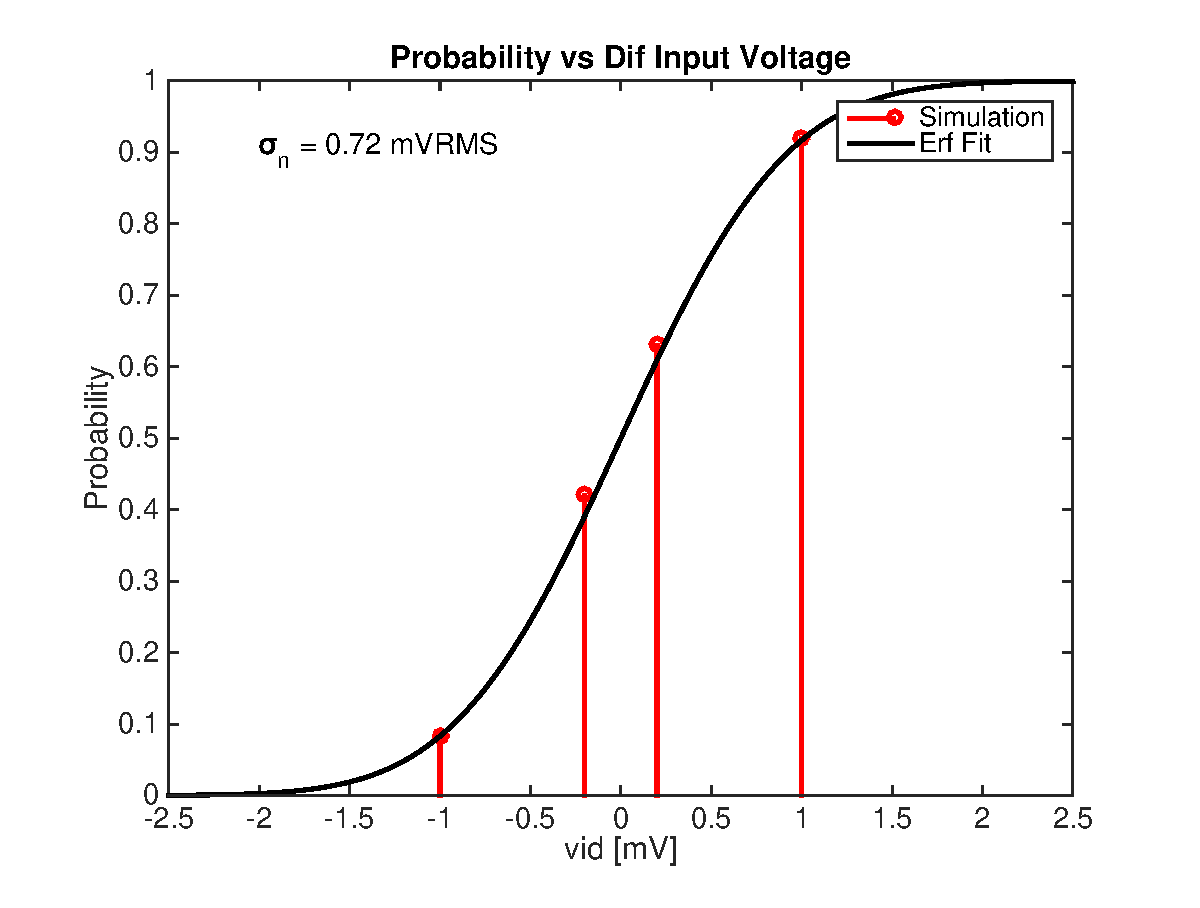
\includegraphics[width=0.6\textwidth]{Part_G.eps}
\caption{Results from transient noise simulation at $\SI{-1}{\milli\volt}$,$\SI{-200}{\micro\volt}$,$\SI{-200}{\micro\volt}$, and $\SI{1}{\milli\volt}$}. 
\label{fig:TransientNoise}
\end{center}
\end{figure}
%%%%%%%%%%%%%%%%%%%%%%%%%%%%%%%%%%%%%%%%%%%%%%%%%%%%%%%%%%%%%%%%%%%%%%%%%%%%%%%
\section{Total DAC Capacitance}
The total DAC capacitance is simply the sum of all the DAC capacitors. In each DAC, there are 9 capacitors, with unit capacitor multipliers ($C_u=\SI{2.5}{\femto\farad}$) of 1, 1, 2, 4, 8, 16, 32, 64, and 128. This gives
\begin{equation}
C_{DAC_{single}}=256C_u=\SI{0.64}{\pico\farad}
\end{equation}
Therefore, the total DAC capacitance for the two DAC configuration is \SI{1.28}{\pico\farad}.

The total sampling noise is simply
\begin{equation}
\overline{v_{n,samp}^2}=\frac{2kT}{C_{DAC_{single}}}\rightarrow\overline{v_{n,samp}}=\SI{0.11}{\mvrms}
\end{equation}


%%%%%%%%%%%%%%%%%%%%%%%%%%%%%%%%%%%%%%%%%%%%%%%%%%%%%%%%%%%%%%%%%%%%%%%%%%%%%%%
\section{SNR}
To calculate the SNR, we must first find the total noise, which we write as
\begin{equation}
\overline{v_{n,total}^2}=\overline{v_{n,quant}^2}+\overline{v_{n,samp}^2}+\overline{v_{n,comp}^2}
\end{equation}
where $\overline{v_{n,samp}^2}$ and $\overline{v_{n,comp}^2}$ were previously calculated. To calculte the sampling noise, we write
\begin{equation}
\overline{v_{n,quant}^2}=\frac{\Delta^2}{12}=\frac{\left(\frac{2V_{ref}}{2^B}\right)^2}{12}\rightarrow\overline{v_{n,quant}}=\SI{0.5638}{\mvrms}
\end{equation}
where $V_{ref}=\SI{1}{V}$. the total noise is then
\begin{equation}
\overline{v_{n,total}}=\SI{0.92}{\mvrms}
\end{equation}
The SNR can be written as
\begin{equation}
SNR=10\log_{10}\left(\frac{P_{sig}}{P_{noise}}\right)
\end{equation}
Assuming a full scale signal from \SI{-1}{\volt} to \SI{1}{\volt}, we find
\begin{equation}
SNR=\SI{57.68}{\decibel}
\end{equation}
\begin{equation}
SQNR=10\log_{10}\left(\frac{P_{sig}}{P_{n,quant}}\right)\SI{61.97}{\decibel}
\end{equation}
%%%%%%%%%%%%%%%%%%%%%%%%%%%%%%%%%%%%%%%%%%%%%%%%%%%%%%%%%%%%%%%%%%%%%%%%%%%%%%%


\end{document}

